Thinking...
The user asks: "以下のの日本語文を英訳してください。ただしTeXのコードが挿入されているのでその部分はそのまま出力してください：" and then provides TeX code: 

\begin{figure}[b] 
\begin{center} 
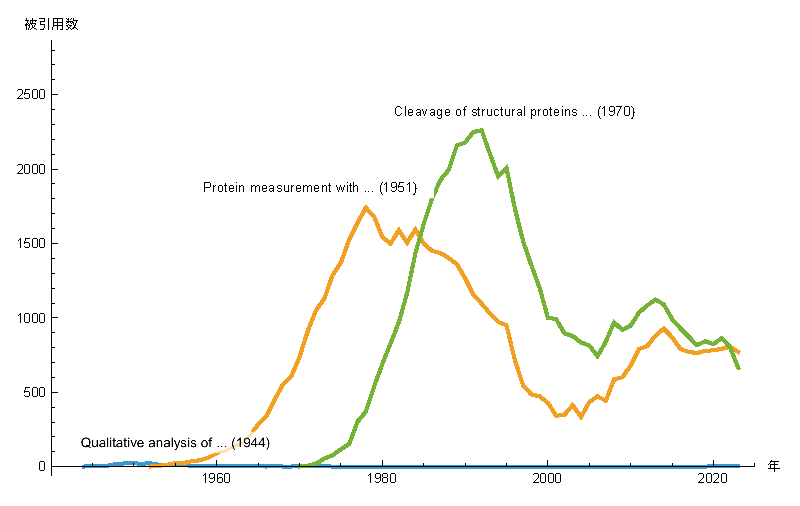
\includegraphics[width=75mm]{nonobscitedplot.eps} 
\caption{最多被引用論文の被引用数の推移} 
\label{fig:nonobs} 
\end{center} 
\end{figure}

They want translation of Japanese text, but preserve TeX code unchanged. The Japanese text is inside caption: "最多被引用論文の被引用数の推移". That translates to something like "Trend of citation counts of the most cited papers". Also perhaps "Trend of the number of citations of the most cited papers". So output should include same TeX code but with caption translated? The instruction says "TeXのコードが挿入されているのでその部分はそのまま出力してください". Means the TeX code should be output as is. However the caption is part of TeX code. Should we translate inside the caption? That is inside TeX code, but it's part of the content. The instruction could mean preserve the TeX syntax but translate the Japanese text inside it. Probably they want the entire snippet with Japanese replaced by English, but keep the TeX commands. So output:

\begin{figure}[b]
\begin{center}
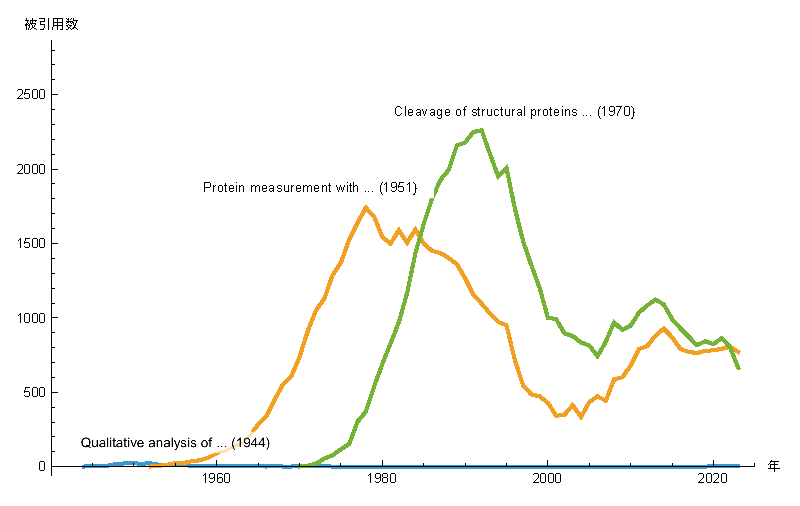
\includegraphics[width=75mm]{nonobscitedplot.eps}
\caption{Trend of citation counts of the most cited papers}
\label{fig:nonobs}
\end{center}
\end{figure}

Thus final answer.
...done thinking.

\begin{figure}[b]
\begin{center}
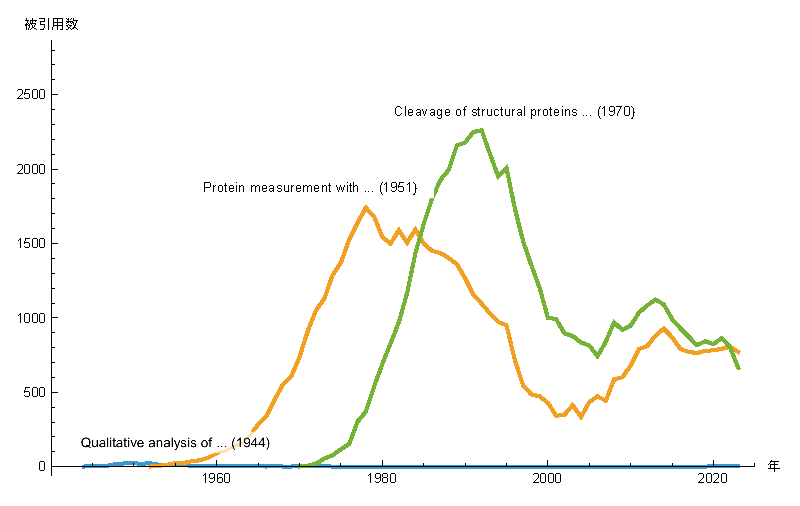
\includegraphics[width=75mm]{nonobscitedplot.eps}
\caption{Trend of citation counts of the most cited papers}
\label{fig:nonobs}
\end{center}
\end{figure}

